% Copyright (c) 2008-2009 solvethis
% Copyright (c) 2010-2016,2018-2019 Casper Ti. Vector
% Public domain.
%
% 使用前请先仔细阅读 pkuthss 和 biblatex-caspervector 的文档,
% 特别是其中的 FAQ 部分和用红色强调的部分。
% 两者可在终端/命令提示符中用
%   texdoc pkuthss
%   texdoc biblatex-caspervector
% 调出。

% 采用了自定义的(包括大小写不同于原文件的)字体文件名,
% 并改动 ctex.cfg 等配置文件的用户请自行加入 nofonts 选项;
% 其它用户不用加入 nofonts 选项,加入之后反而会产生错误。
\documentclass[UTF8, openany]{pkuthss}
% 如果的确须要使脚注按页编号的话,可以去掉后面 footmisc 包的注释。
% 注意:在启用此设定的情况下,可能要多编译一次以产生正确的脚注编号。
%\usepackage[perpage]{footmisc}

% 使用 biblatex 排版参考文献,并规定其格式(详见 biblatex-caspervector 的文档)。
% (如果须要使用作者–年编码制,应将 caspervector 换 成 caspervector-ay)
% 这里按照西文文献在前,中文文献在后排序(“sorting = ecnyt”);
% 若须按照中文文献在前,西文文献在后排序,请设置“sorting = cenyt”;
% 若须按照引用顺序排序,请设置“sorting = none”。
% 若须在排序中实现更复杂的需求,请参考 biblatex-caspervector 的文档。
% \usepackage[backend = biber, style = caspervector, utf8, sorting = none, seconds = true]{biblatex}
\usepackage[backend = biber, style = gb7714-2015, gbnamefmt=lowercase, gbpub=false, doi=false, url=false,eprint=false]{biblatex}

% 对于 linespread 值的计算过程有兴趣的同学可以参考 pkuthss.cls。
\renewcommand*{\bibfont}{\zihao{5}\linespread{1.27}\selectfont}
% 按学校要求设定参考文献列表的段间距。
\setlength{\bibitemsep}{3bp}

% 设定文档的基本信息。
\pkuthssinfo{
	cthesisname = {硕士研究生学位论文 \\ \vspace{1em} 开题报告}, ethesisname = {Master Thesis},
	ctitle = {面向实验室划水的方法研究}, etitle = {Test Document},
	cauthor = {李3号},
	eauthor = {Author Name},
	studentid = {1901213091},
	date = {二〇二一年九月},
	school = {信息工程学院},
	cmajor = {计算机应用技术}, emajor = {Major Name},
	direction = {多媒体信息处理技术},
	cmentor = {某某某教授}, ementor = {Prof.\ Someone},
	ckeywords = {其一,其二}, ekeywords = {First, Second},
	timerange = {2021.09-2021.05}
}
% 载入参考文献数据库(注意不要省略“.bib”)。
\addbibresource{thesis.bib}

% 普通用户可删除此段,并相应地删除 chap/*.tex 中的
% “\pkuthssffaq % 中文测试文字。”一行。
\usepackage{color}
% \def\pkuthssffaq{%
% 	\emph{\textcolor{red}{pkuthss 文档模版最常见问题:}}

% 	\texttt{\string\cite}、\texttt{\string\parencite} %
% 	和 \texttt{\string\supercite} 三个命令分别产生%
% 	上标且带方括号、带方括号的和未格式化的引用标记:%
% 	\cite{test-en},\parencite{test-zh}、\supercite{test-en, test-zh}。

% 	若要避免章末空白页,请在调用 pkuthss 文档类时加入 \texttt{openany} 选项。

% 	如果编译时不出参考文献,
% 	请参考 \texttt{texdoc pkuthss}“问题及其解决”一章
% 	“上游宏包可能引起的问题”一节中关于 biber 的说明。%
% }
\usepackage{multirow}

\begin{document}
	% 以下为正文之前的部分,默认不进行章节编号。
	\frontmatter
	% 此后到下一 \pagestyle 命令之前不排版页眉或页脚。
	\pagestyle{empty}
	% 自动生成封面。
	\maketitle
	% 版权声明。封面要求单面打印,故须新开右页。
	\cleardoublepage
	% \include{chap/copy}

	% 此后到下一 \pagestyle 命令之前正常排版页眉和页脚。
	\cleardoublepage
	\pagestyle{plain}
	% 重置页码计数器,用大写罗马数字排版此部分页码。
	\setcounter{page}{0}
	\pagenumbering{Roman}
	% 中西文摘要。
	% % Copyright (c) 2014,2016 Casper Ti. Vector
% Public domain.

\begin{cabstract}
	\pkuthssffaq % 中文测试文字。
\end{cabstract}

% \begin{eabstract}
% 	Test of the English abstract.
% \end{eabstract}

% vim:ts=4:sw=4

	% 自动生成目录。
	\tableofcontents

	% 以下为正文部分,默认要进行章节编号。
	\mainmatter
	% 各章节。
	% Copyright (c) 2014,2016,2018 Casper Ti. Vector
% Public domain.
% \specialchap{1 引言}
\chapter{引言}

\section{题目及其说明}

本论文题目为《实验室划水谁最在行》。该选题来自于某项目。

如图\ref{fig:water}所示,水(Water)\cite{water}是生命之源。

\begin{figure}[htb]
    \centering
    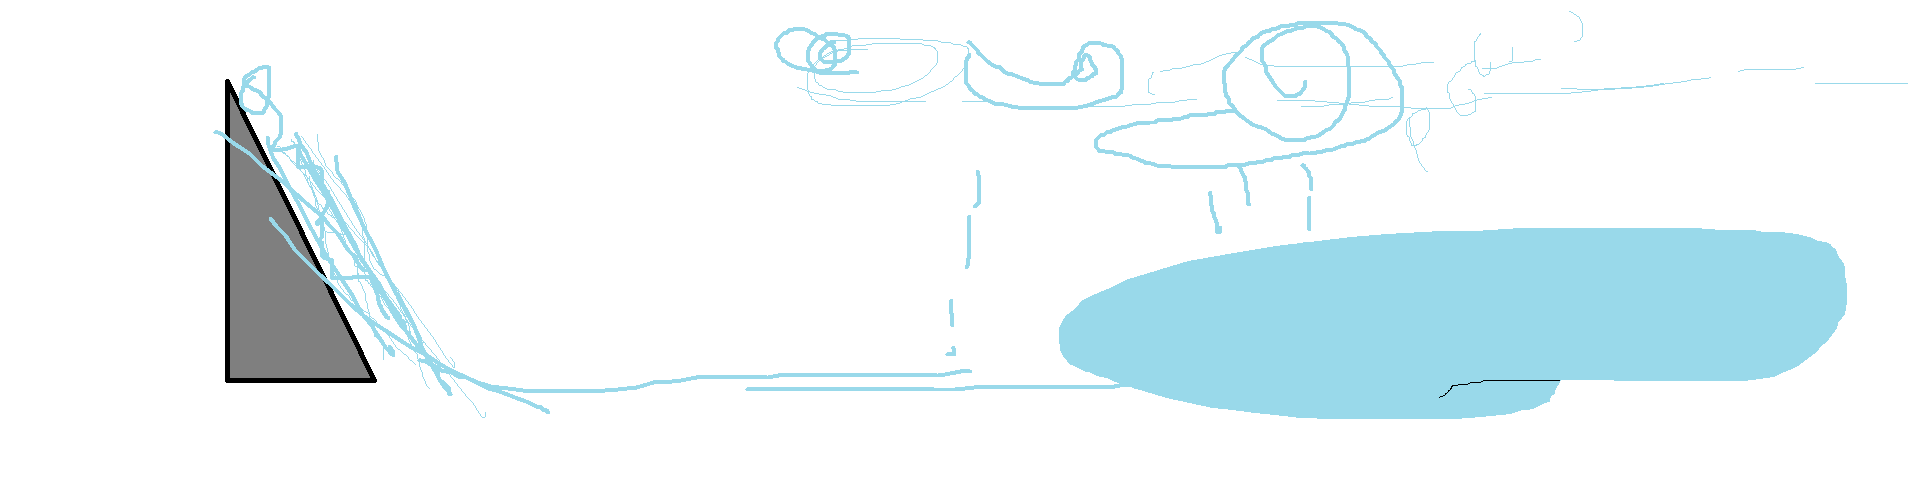
\includegraphics[width=0.9\textwidth]{image/water.png}
    \caption{常见水源}
    \label{fig:water}
\end{figure}


\section{选题的目的、意义及应用前景}

没有意义就是最大的意义。

\section{文献综述}

为了《》课题研究,本人对划水技术进行了调研。

\subsection{视频描述技术的发展}



	% Copyright (c) 2014,2016 Casper Ti. Vector
% Public domain.

\chapter{主要内容}

\section{技术难点}


\subsection{数据偏差问题}
	\chapter{研究方案}

\section{研究方案}



\section{主要实现方法}

\subsection{硬件平台}


\subsection{软件平台}


\subsection{实验数据集}


\subsection{评价标准}

	\chapter{预期目标与成果形式}

\section{预期达到的目标}

本论文设定的预期达到目标包括:


\noindent(1)设计一种划水方法,避免被老板发现。

\noindent(2)发表高质量的国内外研究论文(EI/SCI收录)1-2篇;


\section{成果形式}

\noindent(1)预期研究目标所述系统与算法的Python代码;

\noindent(2)1-2篇研究论文;

\noindent(3)1项国内发明专利。

	\chapter{目前取得的主要进展}


\section{整体框架}


\begin{equation} 
    % \label{}
    W = H_2O
\end{equation}
其中$W$为Water.


\begin{table}[ht]
    \caption{不同水源表现对比}
    \centering
    \begin{tabular}{ccccc}
    \toprule
    \textbf{水源} & \textbf{水质} \\
    \midrule
    自来水 & 一般 \\
    矿泉水 & 能喝 \\
    \bottomrule
    \end{tabular}
    \label{tab:water}
\end{table}

如表\ref{tab:water}所示,矿泉水一般能喝。
	\chapter{研究计划与进度安排}

\section{第三学年上学期}

\noindent 1)2021/11/01-2021/11/30:完成死水考察的实验;

\noindent 2)2021/12/01-2021/12/31:针对坏水考察的研究,设计坏水样本的方法,并进行实验与性能分析;

\noindent 3)2022/01/01-2022/01/31:完成研究论文一篇。

\section{第三学年下学期}

\noindent 1)2022/02/21-2022/05/01: 撰写硕士学位论文;

\noindent 2)2022/05/01-2022/05/31: 准备硕士学位论文答辩;

\noindent 3)2022/06/01-2022/06/30: 完成实验室科研工作交接。
	\chapter{工作基础}

\section{团队工作基础}

整体氛围好。

\section{本人工作基础}

常年划水。

{
\let\clearpage\relax
\let\cleardoublepage\relax

\vspace{1cm}
\chapter{个人简介}

% \noindent
\begin{minipage}{0.13\linewidth}
    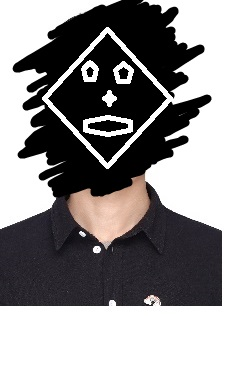
\includegraphics[width=\linewidth]{image/avatar.jpg}
    \end{minipage}
    \hfill
    \begin{minipage}{0.87\linewidth}
        李3号,男,某省某市人,学号:1901213000 \\
        研究方向:多媒体信息处理技术、自然语言处理、某某方法 \\
        2019–至今~北京大学~信息工程学院~计算机应用技术 \\
        2015–2019~京北大学~计算机与通信工程学院~计算机科学与技术 \\
\end{minipage}

}



	% 正文中的附录部分。
	% \appendix
	% 排版参考文献列表。bibintoc 选项使“参考文献”出现在目录中;
	% 如果同时要使参考文献列表参与章节编号,可将“bibintoc”改为“bibnumbered”。
	\printbibliography[heading = bibintoc]
	% 各附录。
	% \include{chap/encl1}

	% 以下为正文之后的部分,默认不进行章节编号。
	\backmatter
	% 致谢。
	% \include{chap/ack}
	% 原创性声明和使用授权说明。
	% \include{chap/origin}
\end{document}

% vim:ts=4:sw=4